\documentclass[18pts]{article}
\usepackage{amssymb,amsmath,latexsym,enumerate,graphicx,fullpage,url,multicol,longtable,color}
\usepackage{graphicx, tikz}
\usetikzlibrary{calc,shadows}
\usepackage[T1]{fontenc}
\usepackage{eso-pic,fancybox}
\usepackage[absolute,overlay]{textpos}
\usepackage{color}
\usepackage{mathptmx}
\usepackage{fix-cm}
\graphicspath{ {images/} }
%    \topmargin 0 in
%    \textheight 11in
%    \textwidth 6.25 in
%    \oddsidemargin 1in   % read Lamport p.163
%    \evensidemargin 1 in
%    \headsep = 20pt
\usepackage{anyfontsize}
\usepackage{xparse}

% suppresses hyphenation and aligns left
\usepackage[none]{hyphenat}
\raggedright


\newcommand\ProjectName[1]{
{
\fontsize{35}{40}\selectfont
\noindent\textbf{#1}\par
}
\vskip 2mm
\fontsize{20}{25}\selectfont
}

\newenvironment{justified}
{
\tolerance=1
\emergencystretch=\maxdimen
\hyphenpenalty=10000
\hbadness=10000
}


\renewcommand\large{
\noindent\fontsize{16}{19}\selectfont}
\renewcommand\Large{
\noindent\fontsize{18}{20}\selectfont}


%%%%%%%%%%%%%%%%%%%%%%%%%%%%%%%%%%%%%%%%%%%%%%%%%%%%%%
%
%					DO NOT CHANGE ANY ABOVE FORMAT/MACRO
%
%%%%%%%%%%%%%%%%%%%%%%%%%%%%%%%%%%%%%%%%%%%%%%%%%%%%%%

\begin{document}

\ProjectName{Automata and\\ Numeration Systems}
\noindent\textbf{Faculty Mentors: {Philipp Hieronymi \& Erik Walsberg}
}
\vskip 2mm
\noindent\textbf{Team Leaders: {Eion Blanchard \& Alexi Block Gorman}}
\vskip 2mm
\noindent\textbf{Scholars: Jack Gentile, Erik Joan Hernandez, Dun ``Eric'' Ma, Steve O'Brien, \& Haozhe ``Howard'' Wang}
\\
\vskip 2mm
\Large

\begin{justified}
Irrational numbers can be represented as sets of natural numbers by way of continued fraction expansions. These sets repeat with small period, and an Ostrowski numeration system uses such an expansion to calculate base values. Using algorithms put forth in Hieronymi and Terry's paper "Ostrowski Numeration Systems," we generated an automaton that adds numbers in this type of representation. \\
We then used the theorem-proving software Walnut to express logical statements in Ostrowski numeration systems in order to mimic results from Du, Mousavi, Schaeffer, and Shallit's paper "Decision Algorithms for Fibonacci-Automatic Words, with Applications to Pattern Avoidance" for more general words.

\end{justified}


\begin{figure}[h!]
\vspace{10mm}
	\begin{minipage}{0.4\textwidth}
      \centering
      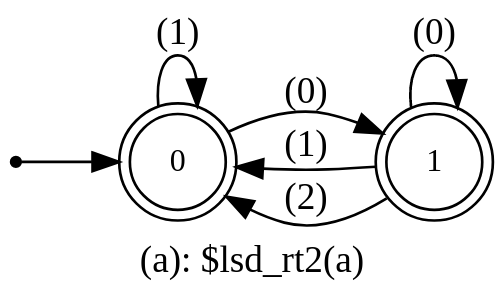
\includegraphics[width=\linewidth]{lsd_rt2.png}
      \centering

  	\end{minipage}%
    \hspace{0.05\textwidth}
    \begin{minipage}{0.55\textwidth}
      \centering
      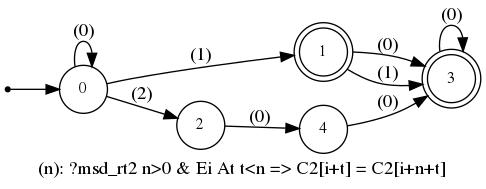
\includegraphics[width=\linewidth]{theorem6_gv.jpg}
      \centering

    \end{minipage}
\end{figure}




\end{document} 